\begin{figure}[tp]
  \centering
  {\fontfamily{pag}\selectfont  
  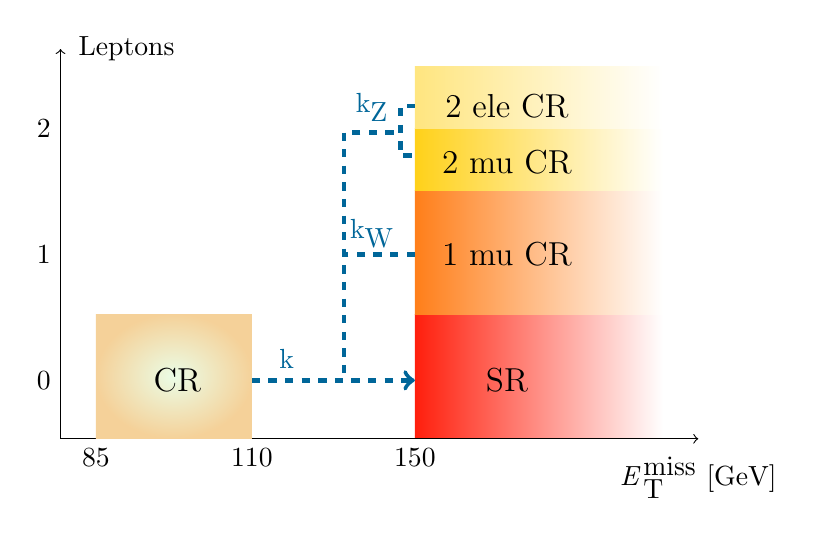
\begin{tikzpicture}[scale=0.9]

      \draw [->](0,0)--(9,0) node[below=3pt]{{\itshape E}$\,_\textup{T}^\textup{miss}$ [GeV]} ;
      \draw [->](0,0)--(0,5.5)node[right=3pt]{Leptons};
      
      \draw node [left] at(0,0.825) {0};
      \draw node [left] at(0,2.6) {1};
      \draw node [left] at(0,3.5+1.75/2) {2};
      \draw node [below] at(0.5,0) {85};
      \draw node [below] at(2.7,0) {110};
      \draw node [below] at(5,0) {150};

      \shade[left color =orange!15!red!95, right color=white] (5,0.015) rectangle +(3.5,1.75-0.015);
      \node[] at (6.3,0.825){\large SR};
      \shade[left color =red!60!yellow!60!orange!90, right color=white] (5,1.75) rectangle +(3.5,1.75);
      \node[] at (6.3,2.6) {\large 1 mu CR};
      \shade[left color =red!20!yellow!90, right color=white] (5,3.5) rectangle +(3.5,1.75/2);
      \node[] at (6.3,3.9) {\large 2 mu CR};
      \shade[left color =orange!40!yellow!50, right color=white] (5,3.5+1.75/2) rectangle +(3.5,1.75/2);
      \node[] at (6.3,4.7) {\large 2 ele CR};
      \shade[outer color=orange!90!green!40,inner color=orange!20!green!10] (0.5,0.01) rectangle +(2.2,1.75);
      \node[align=left] at (1.65,0.825) {\large \gammajet CR};
      
      
      \draw[ultra thick,dashed,->,green!40!blue!100] (2.7,0.825)--(5,0.825);
      \draw node[green!40!blue!100] at (3.2,1.1){k$_{\gammajet}$};
      
      \draw[ultra thick,dashed,green!40!blue!100] (5,4.7)--(4.8,4.7)--(4.8,4)--(5,4);
      \draw[ultra thick,dashed,green!40!blue!100] (4.7,3.5+1.75/2-0.05)--(4,3.5+1.75/2-0.05)--(4,0.87);
      \node[green!40!blue!100] at (4.4,3.5+1.75/2+0.3) { k$_{\textup{Z}}$};
      
      \draw[ultra thick,dashed,green!40!blue!100] (5,2.6) -- (4,2.6);
      \node[green!40!blue!100] at (4.4,2.9) { k$_{\textup{W}}$};
    
   
  \end{tikzpicture}
  }
  \caption{Visual representation of the cuts on \met and number of leptons required for the SR and CRs. The normalization factors k$_\textup{i}$ extracted from CRs and applied to the SR are also shown.}
  \label{fig:regions}
\end{figure}